\documentclass[12pt,letterpaper]{article}
\usepackage{amsmath}
\usepackage{amsfonts}
\usepackage{amssymb}
\usepackage{enumitem}
\usepackage[left=2cm,right=2cm,top=3cm,bottom=3cm]{geometry}
\usepackage{natbib}
\usepackage{graphicx}
\usepackage{hyperref}

\def\wl{\par \vspace{\baselineskip}}

\author{Abel Flores Prieto}
\title{Casptone Project Write Up - Cosmic Microwave Background Data}

\begin{document}
\maketitle

\section{Scope}
This project focuses on the data used for computing the Cosmic Microwave
Background or CMB. In this project I focus to easily enable access to data used
for computing the CMB. The data used for this project is simulated by
href{https://arxiv.org/abs/0908.0540}{Sehgal et al. (2010)} and can be found
\href{https://lambda.gsfc.nasa.gov/simulation/tb\_sim\_ov.cfm}{here}.



% Sample figure
\begin{figure}[h!]
    \centering
    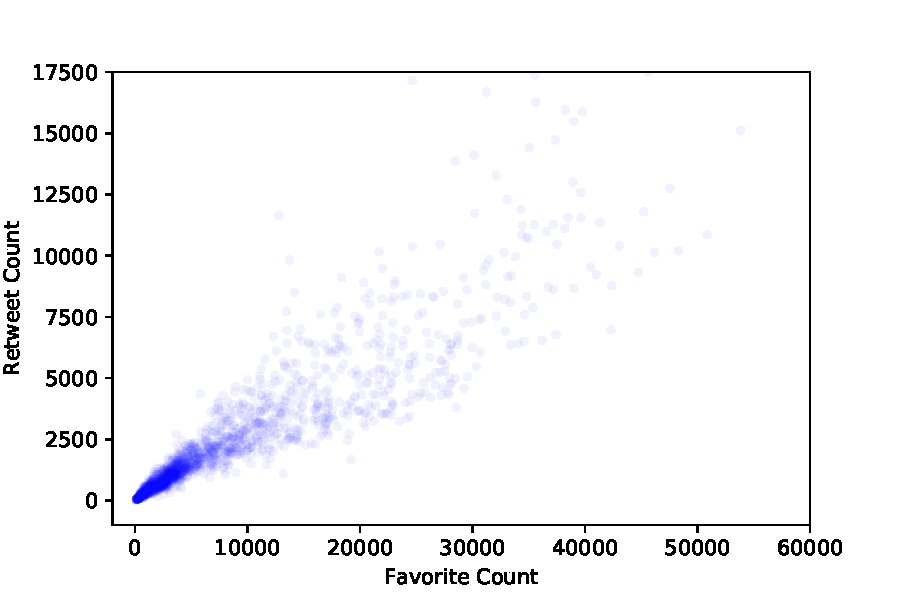
\includegraphics[width=0.75\textwidth]{imgs/sample_figure.pdf}
    \caption{\label{fig:test}Histogram for the confidence percent for
    the prediction of tweet image.}
\end{figure}
% to ref figure do \ref{fig:test}

\end{document}
